\section{Resolución por \textit{Backtracking}}
	\subsection{Descripción del algorítmo}

	La solución por Bactracking emplea recursividad en cada paso, y recorre el espacio de soluciones como si el mismo fuese un arbol en preorden.

	\begin{algorithm}[H]
		\KwData{Lista, la lista de números a pintar}

		\KwData{UltRojo, la posición del úlitmo rojo que pintamos (si existe)}

		\KwData{UltAzul, la posición del úlitmo azul que pintamos (si existe)}

		\KwData{Indice, la posición que estamos mirando ahora (0 si recién empezamos)}

		\KwData{Res, la cantidad de elemntos no pintados hasta ahora (0 si recién empezamos)}

		\eIf{Indice es igual al tamaño de Lista}{
			Llegamos al final de la lista, no hacer nada
		}{
			Calcular el mejor resultado sin pintar

			Llamada Recursiva aumentando Indice y Res en 1, y conservando los otros parámetros

			Guardar ese resultado como Res

			\If{no existe UltRojo o es menor que Lista[Indice]}{
				Calcular el mejor resultado pintando de Rojo

				Llamada Recursiva cambiando UltRojo por Lista[Indice], aumentando Indice en 1 y conservando los otros parámetros

				Si ese resultado es menor que Res, guardarlo como Res
			}
			\If{no existe UltAzul o es mayor que Lista[Indice]}{
				Calcular el mejor resultado pintando de Azul

				Llamada Recursiva cambiando UltAzul por Lista[Indice], aumentando Indice en 1 y conservando los otros parámetros

				Si ese resultado es menor que Res, guardarlo como Res
			}
		}

		\KwResult{Res}
	\end{algorithm}

	Cabe destacar que el orden en que se calculan los posibles resultados no es relevante, en tanto se conserve el menor de todos.

	\subsection{Cota de complejidad}

	El algoritmo propuesto realiza hasta tres llamadas recursivas en cada paso (asumiendo que el próximo número se puede pintar de cualquier color). Esto siempre es cierto para los primeros dos elementos.

	En el mejor caso, en cualquier paso se llama solo una llamada recursiva (no se puede pintar el número).

	En cualquier llamada recursiva, el tamaño del problema a resolver disminuye en 1 (se avanza/pinta un solo número).

	La función de complejidad sería
	\[
	T(BT(n)) =
		\begin{cases}
			\text{1,} &\quad\text{si n == 0}\\
			\text{3 T(BT(n-1)),} &\quad\text{si no} \\
		\end{cases}
	\]

	donde n es la cantidad de números restantes, es decir, $|Lista| - Indice$.

	Como, en peor caso, el algorítmo realiza 3 llamadas recursivas n veces, la complejidad resultante es \textbf{O($3^n$)}, donde n es el largo de la lista de números de entrada (es decir, cuántos numeros contiene la lista).

	\pagebreak
	\subsection{Gráfico de complejidad}

	El siguiente gráfico muestra la relación entre la cantidad de elementos y el tiempo que el algoritmo toma en resolver el problema. Para el mismo se utilizaron listas con contenido random, ignorando el resultado real de las mismas. A su vez, cada caso se corrió 20 veces para tratar de reducir el ruido generado por otras aplicaciones corriendo en el equipo.

	Los tiempos fueron medidos con las utilidades de \texttt{std::chrono} de C++11, corriendo dentro de los equipos de los laboratorios del DC.

	Como se puede apreciar, el tiempo crece muy rápidamente con respecto al tiempo. Originalmente las mediciones estaban en microsegundos ($seg \times 10^{-6}$), pero fueron escaladas a segundos para este caso. Casos de tamaño mayor a 50 no fueron testeados por el gran costo temporal asociado con esos tests.

	\begin{center}
	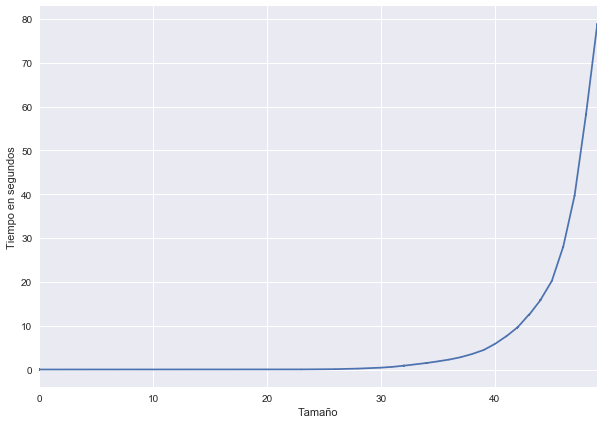
\includegraphics[width=.8\textwidth]{ej1.png}
	\end{center}